\documentclass{book}
\usepackage[left=2cm, right=2cm, top=2cm, bottom=2cm]{geometry}

\usepackage[spanish]{babel}
\usepackage[utf8]{inputenc}

\usepackage{pdfpages}
\usepackage{hyperref} % Para enlaces y metadatos
\usepackage{fontawesome5}
\usepackage{fancyhdr}
\usepackage{bookmark}

\hypersetup{
    colorlinks=true,
    linkcolor=black,  % Color de los enlaces internos (por ejemplo, dentro de la tabla de contenidos)
    urlcolor=magenta,   % Color de los enlaces a URLs
    %%citecolor=green,
    pdfauthor={Moisés Serrano Samudio},
    pdftitle={Villancicos Populares},
    pdfsubject={partituras},
    pdfkeywords={violín,trío,villancicos}
}

\title{Villancicos Populares}
\author{Moisés Serrano Samudio}
\date{24 octubre 2023}

\begin{document}

\setcounter{page}{1}

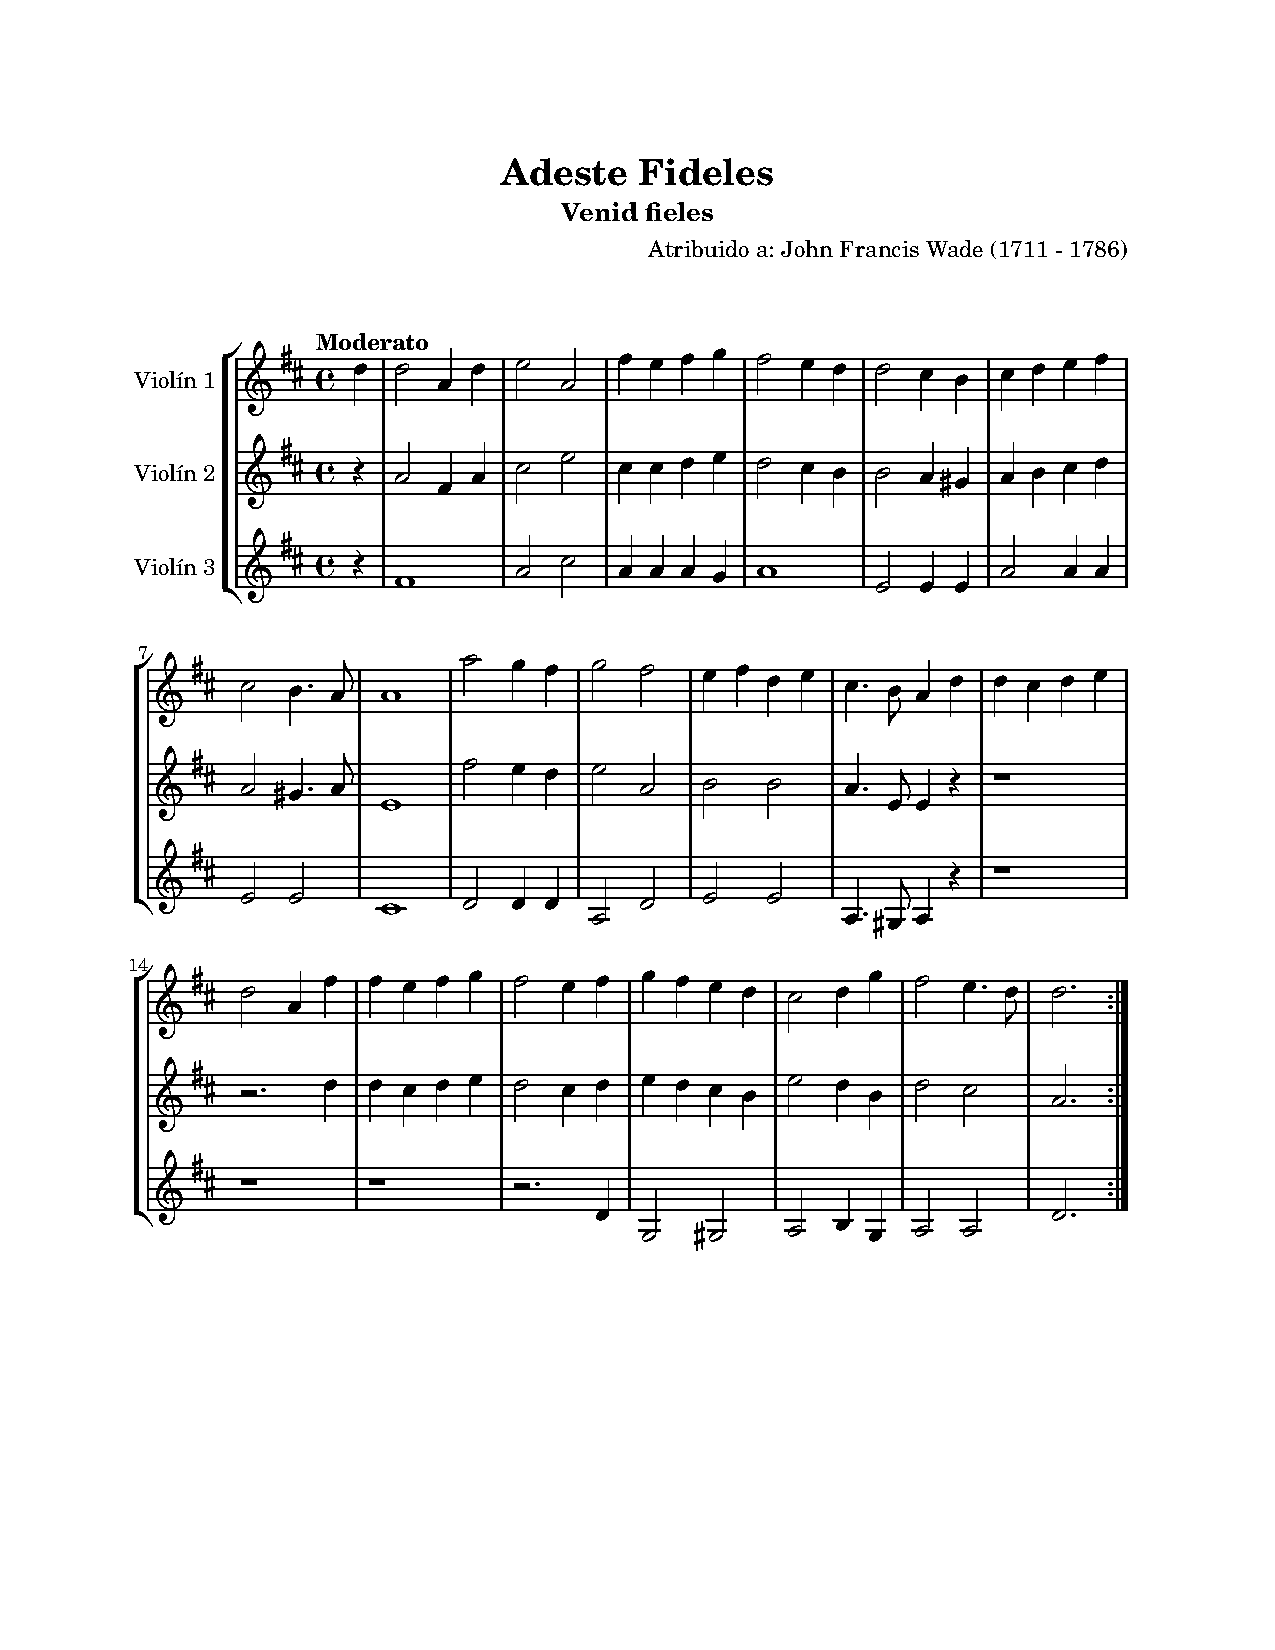
\includepdf[pages=-, pagecommand={\thispagestyle{plain}}]{adeste-fideles.pdf}

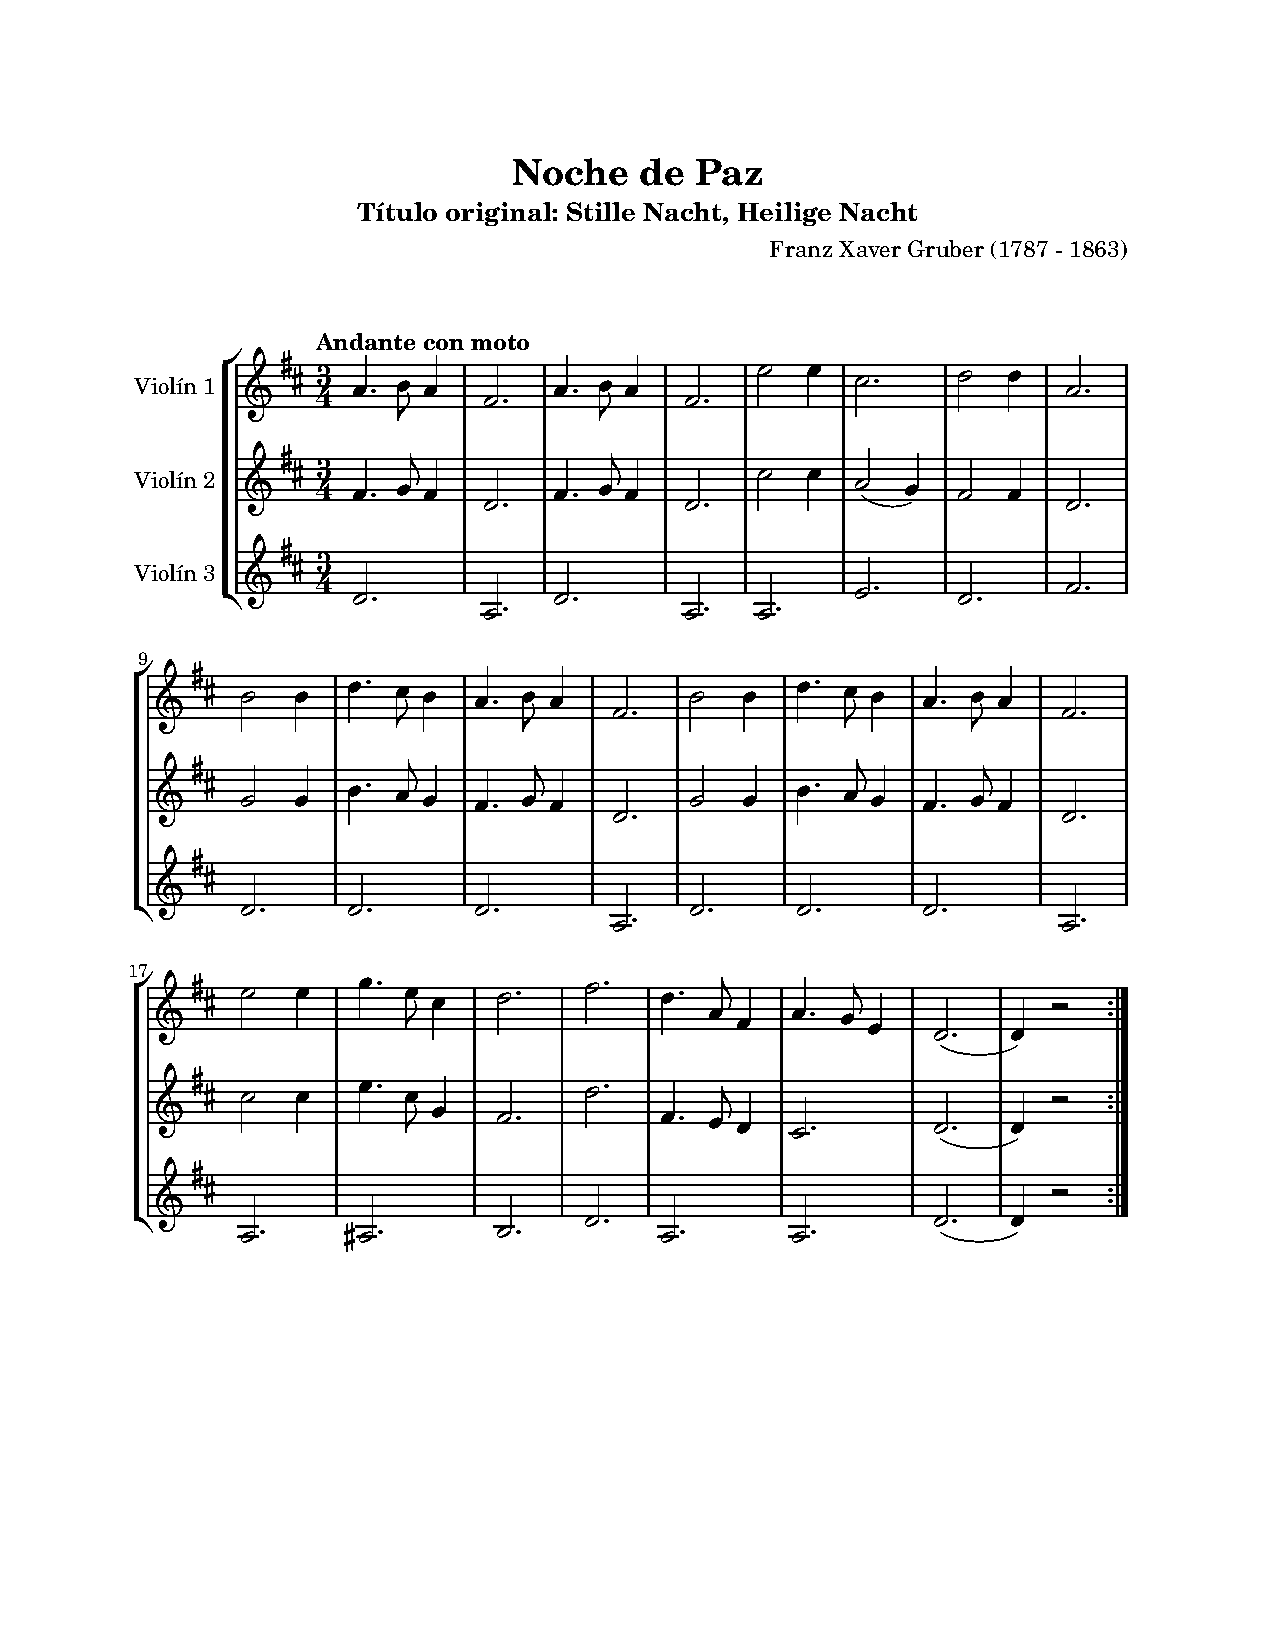
\includepdf[pages=-, pagecommand={\thispagestyle{plain}}]{noche-de-paz.pdf}

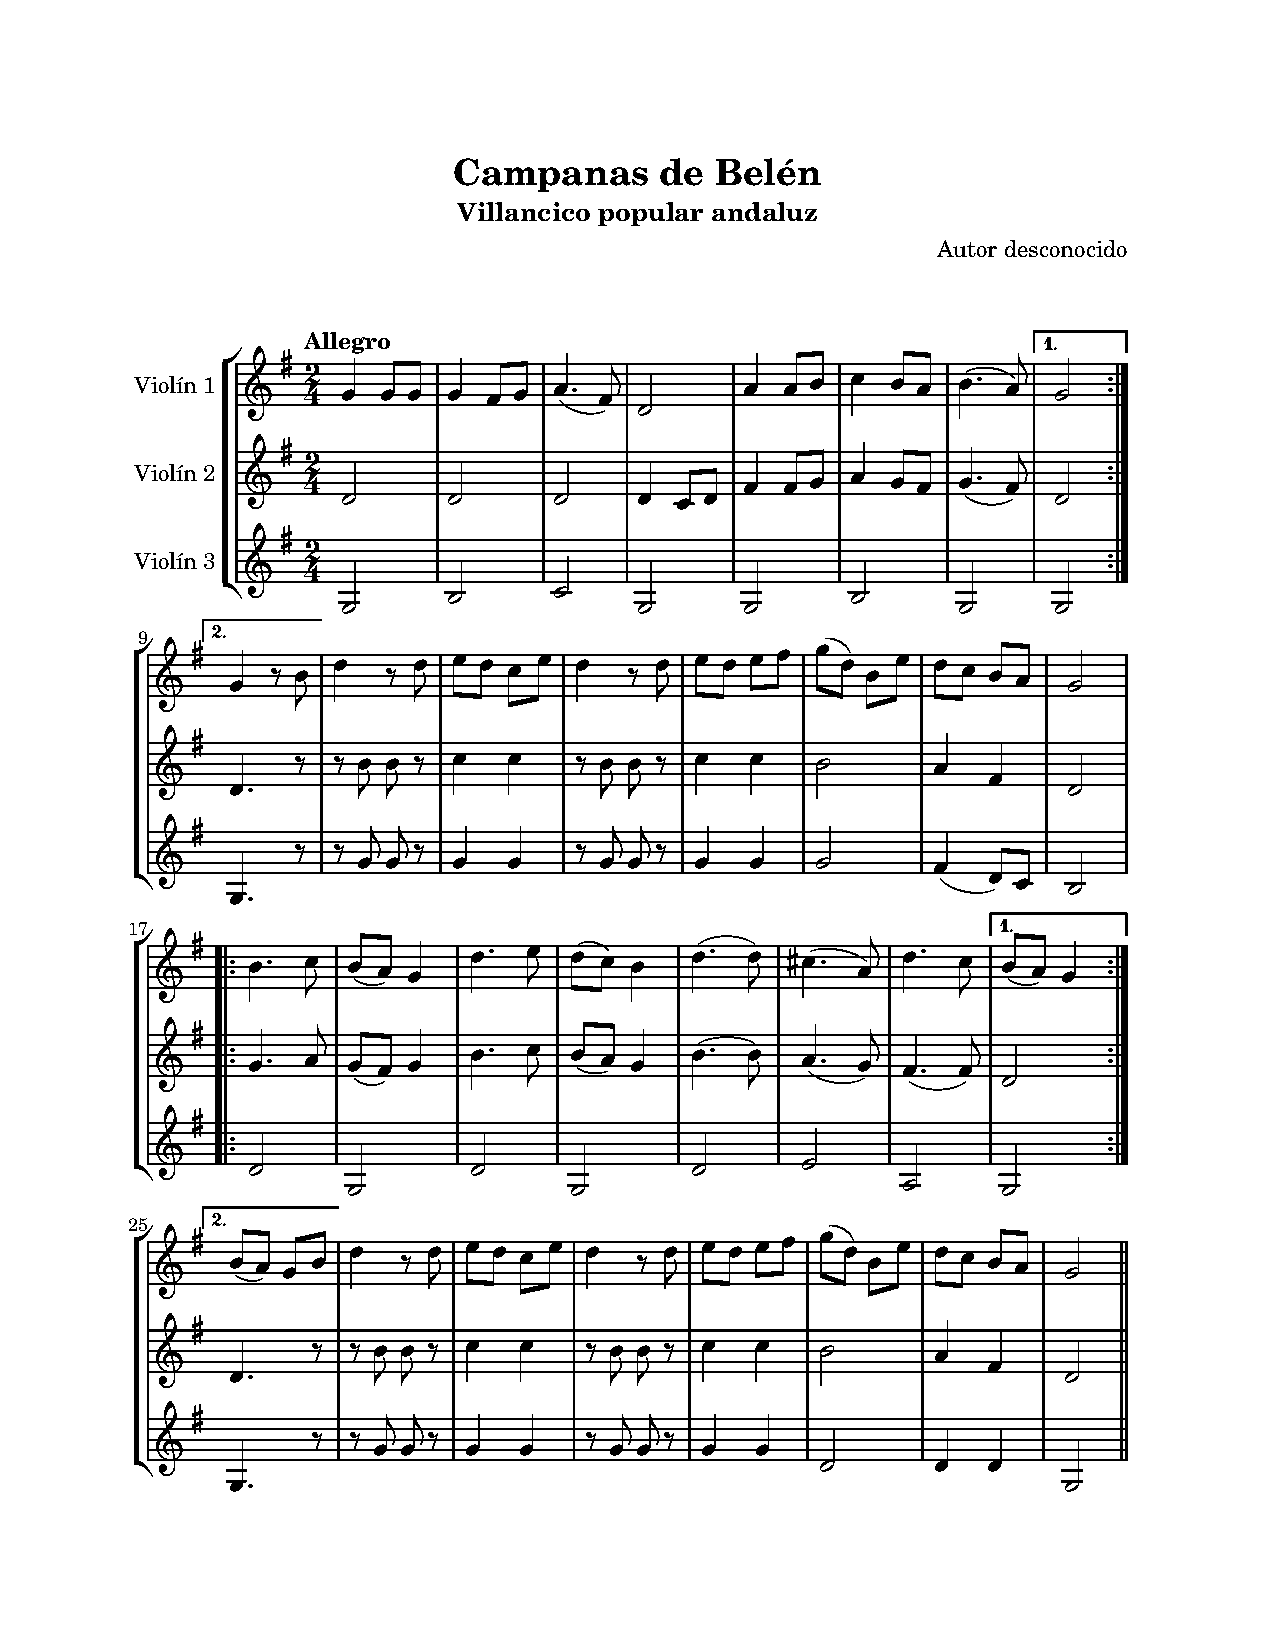
\includepdf[pages=-, pagecommand={\thispagestyle{plain}}]{campanas-de-belen.pdf}

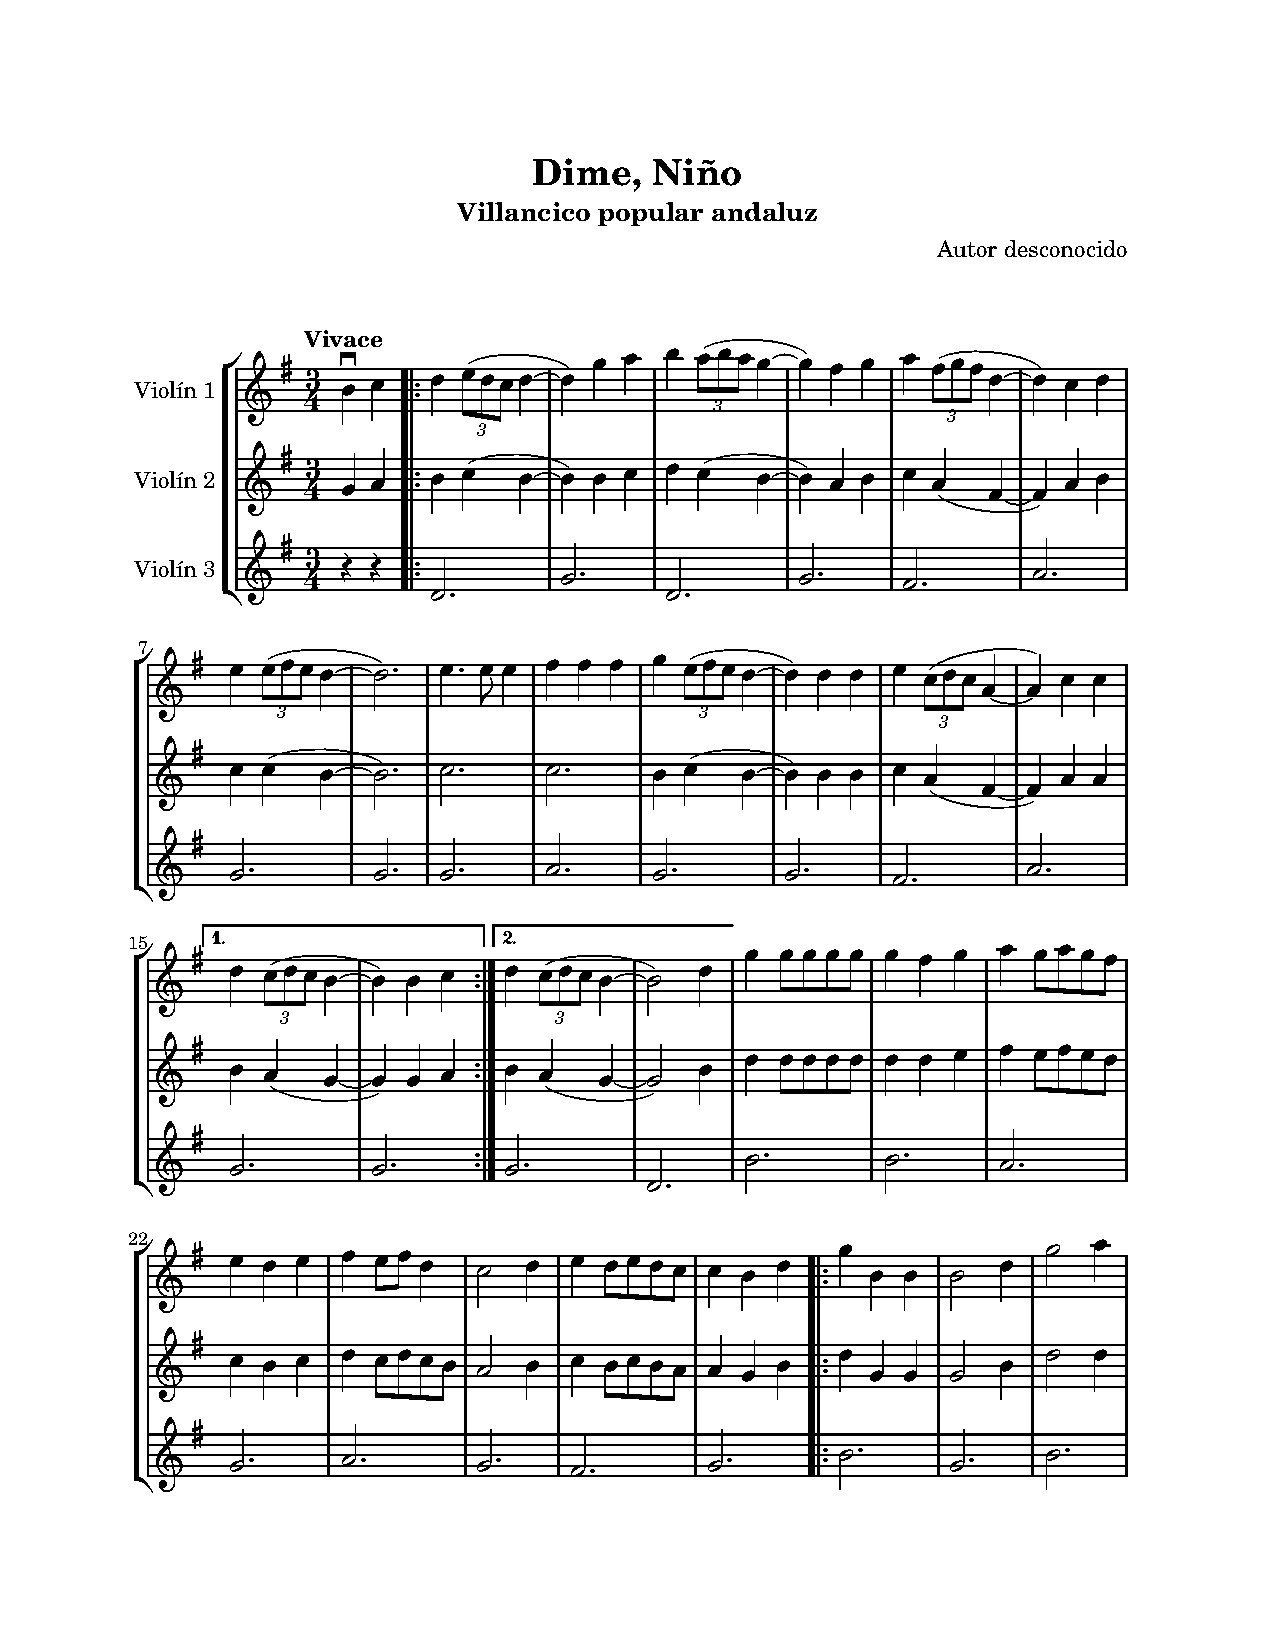
\includepdf[pages=-, pagecommand={\thispagestyle{plain}}]{dime-niño.pdf}

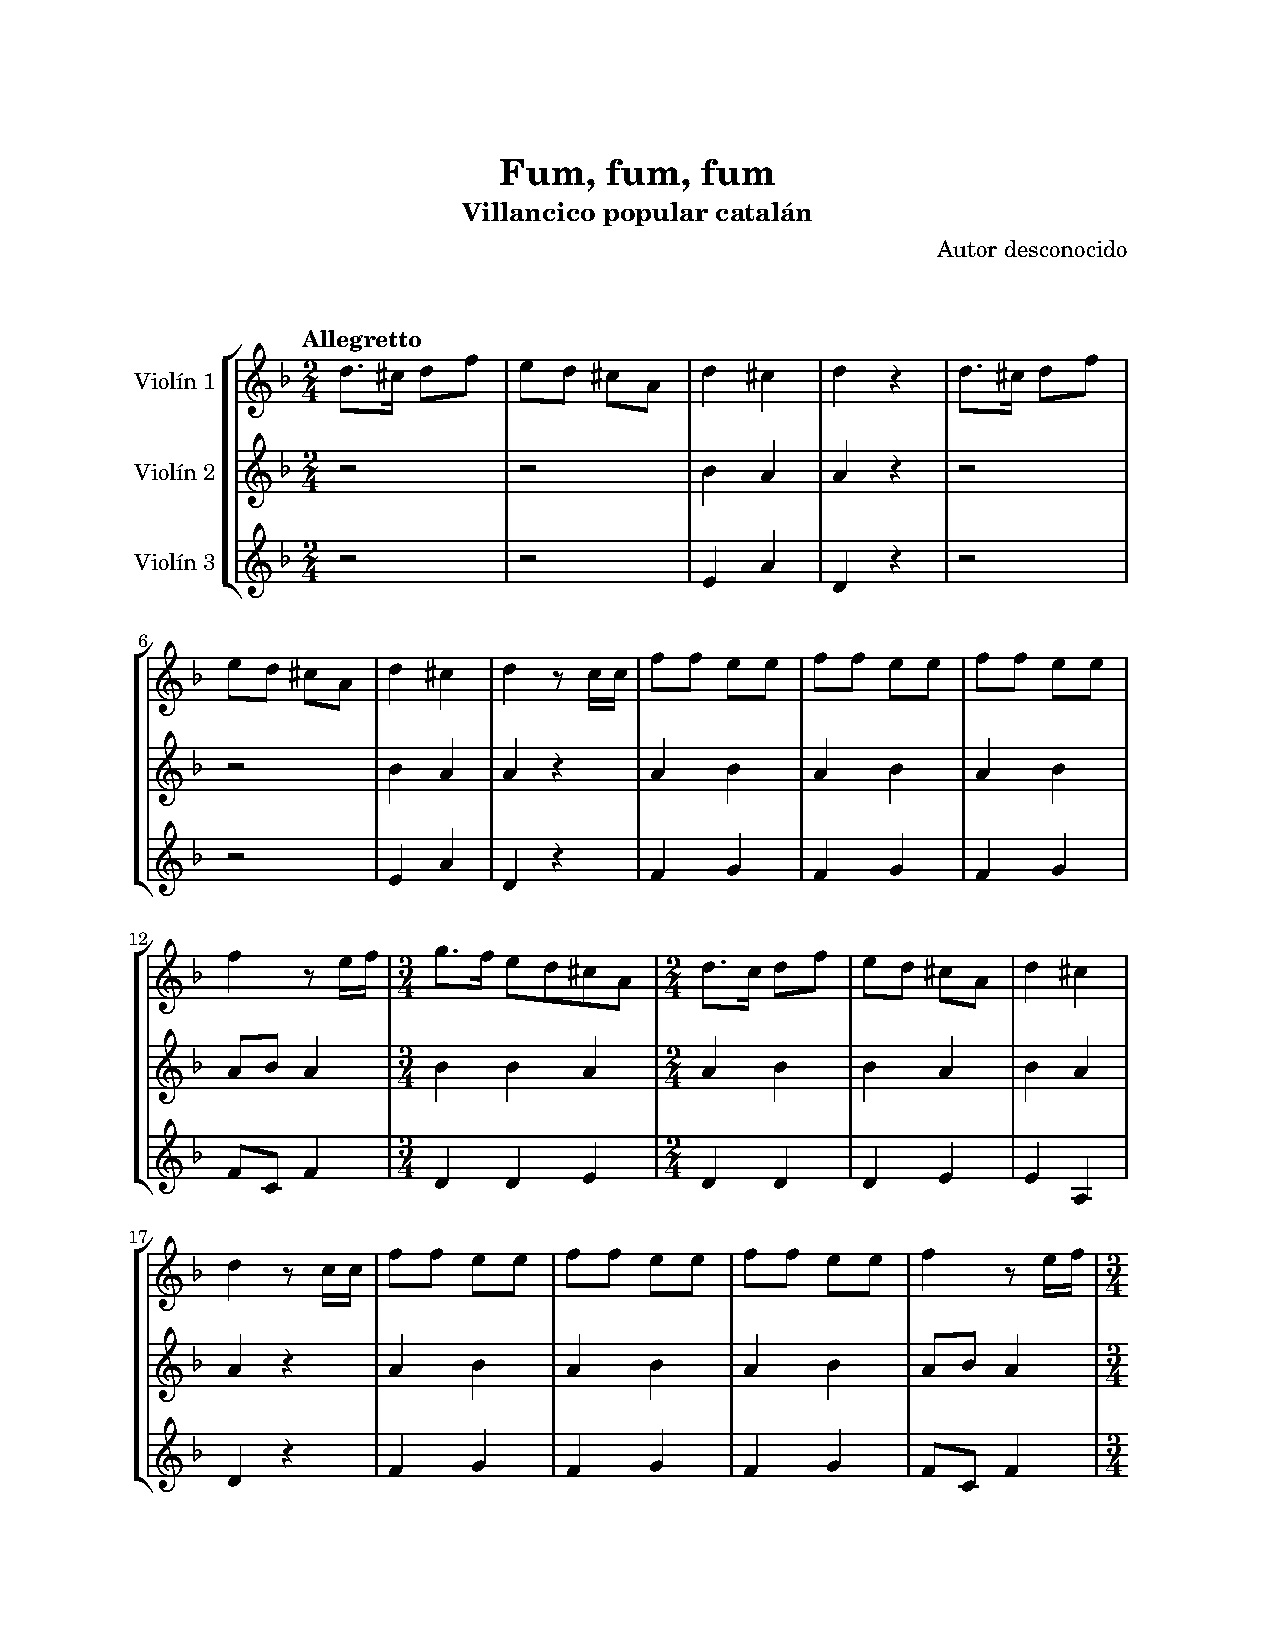
\includepdf[pages=-, pagecommand={\thispagestyle{plain}}]{fum-fum-fum.pdf}

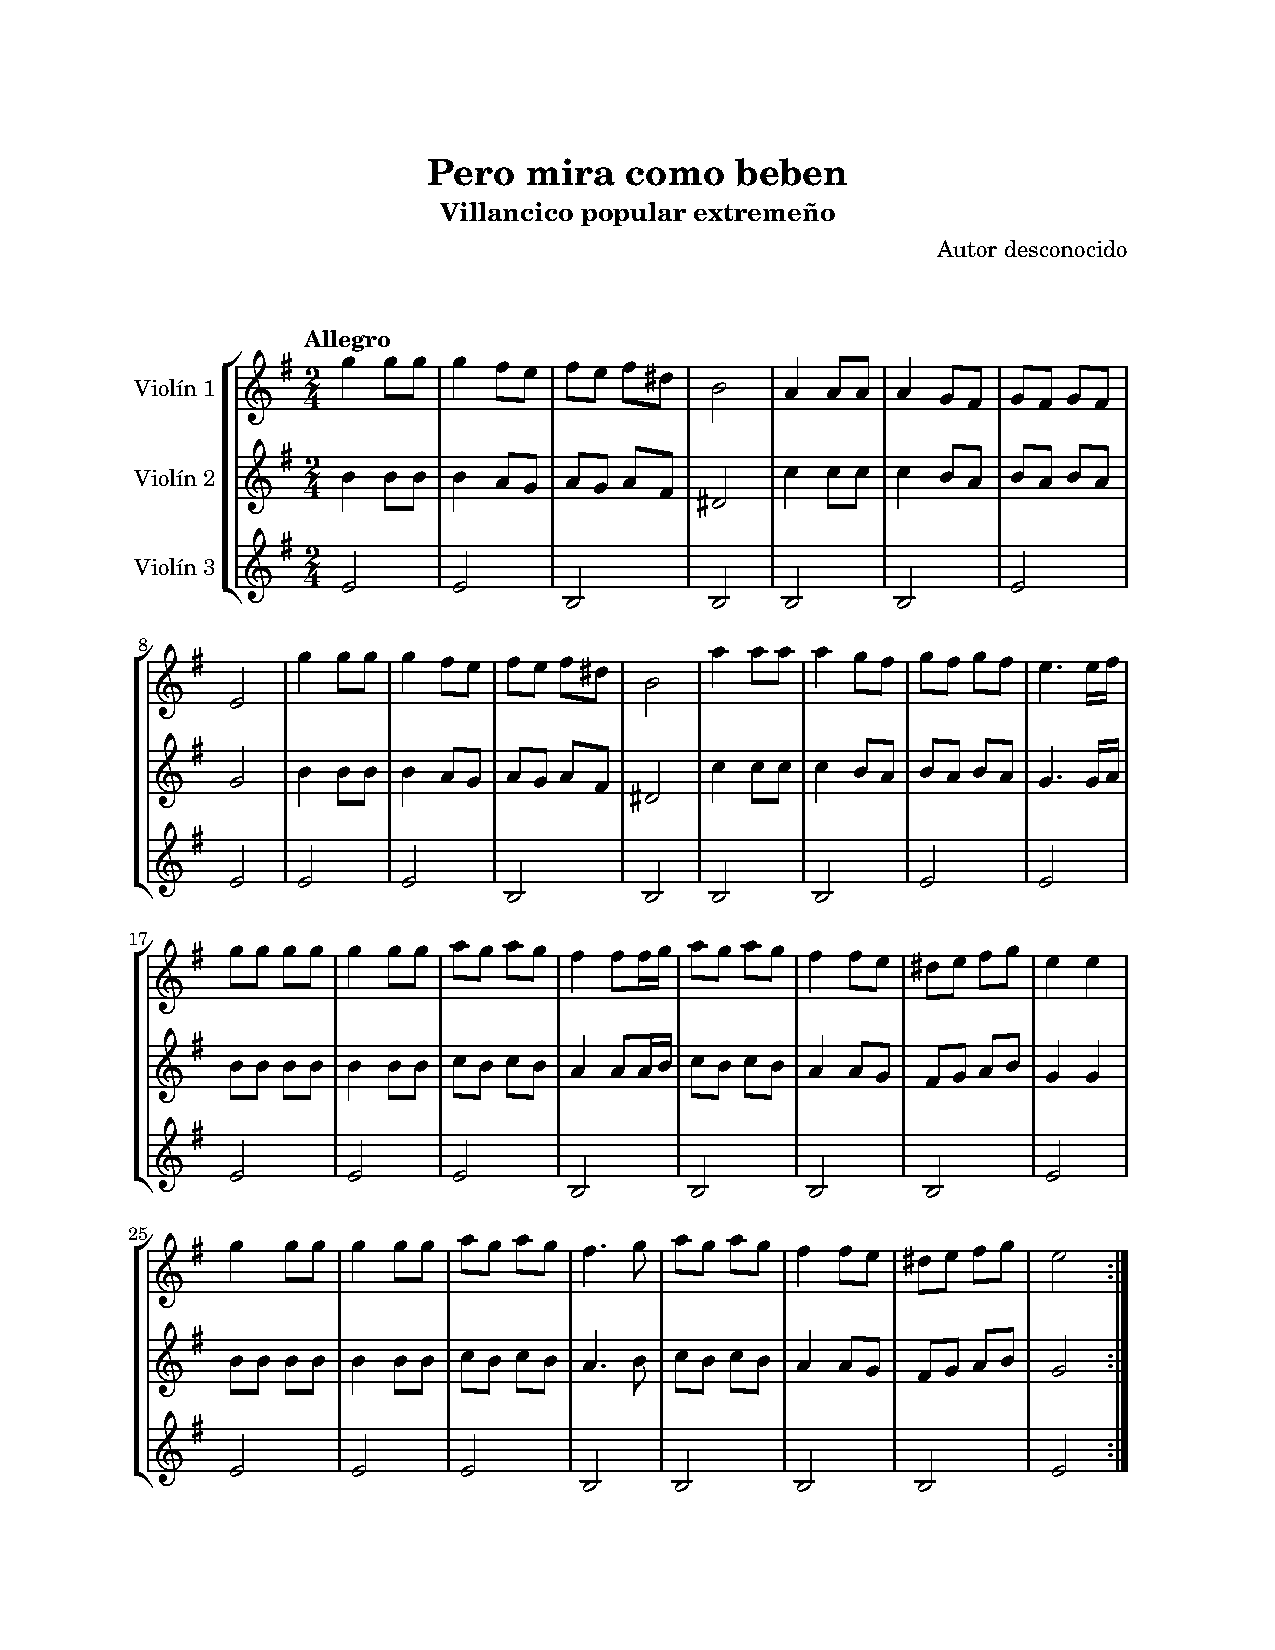
\includepdf[pages=-, pagecommand={\thispagestyle{plain}}]{pero-mira-como-beben.pdf}

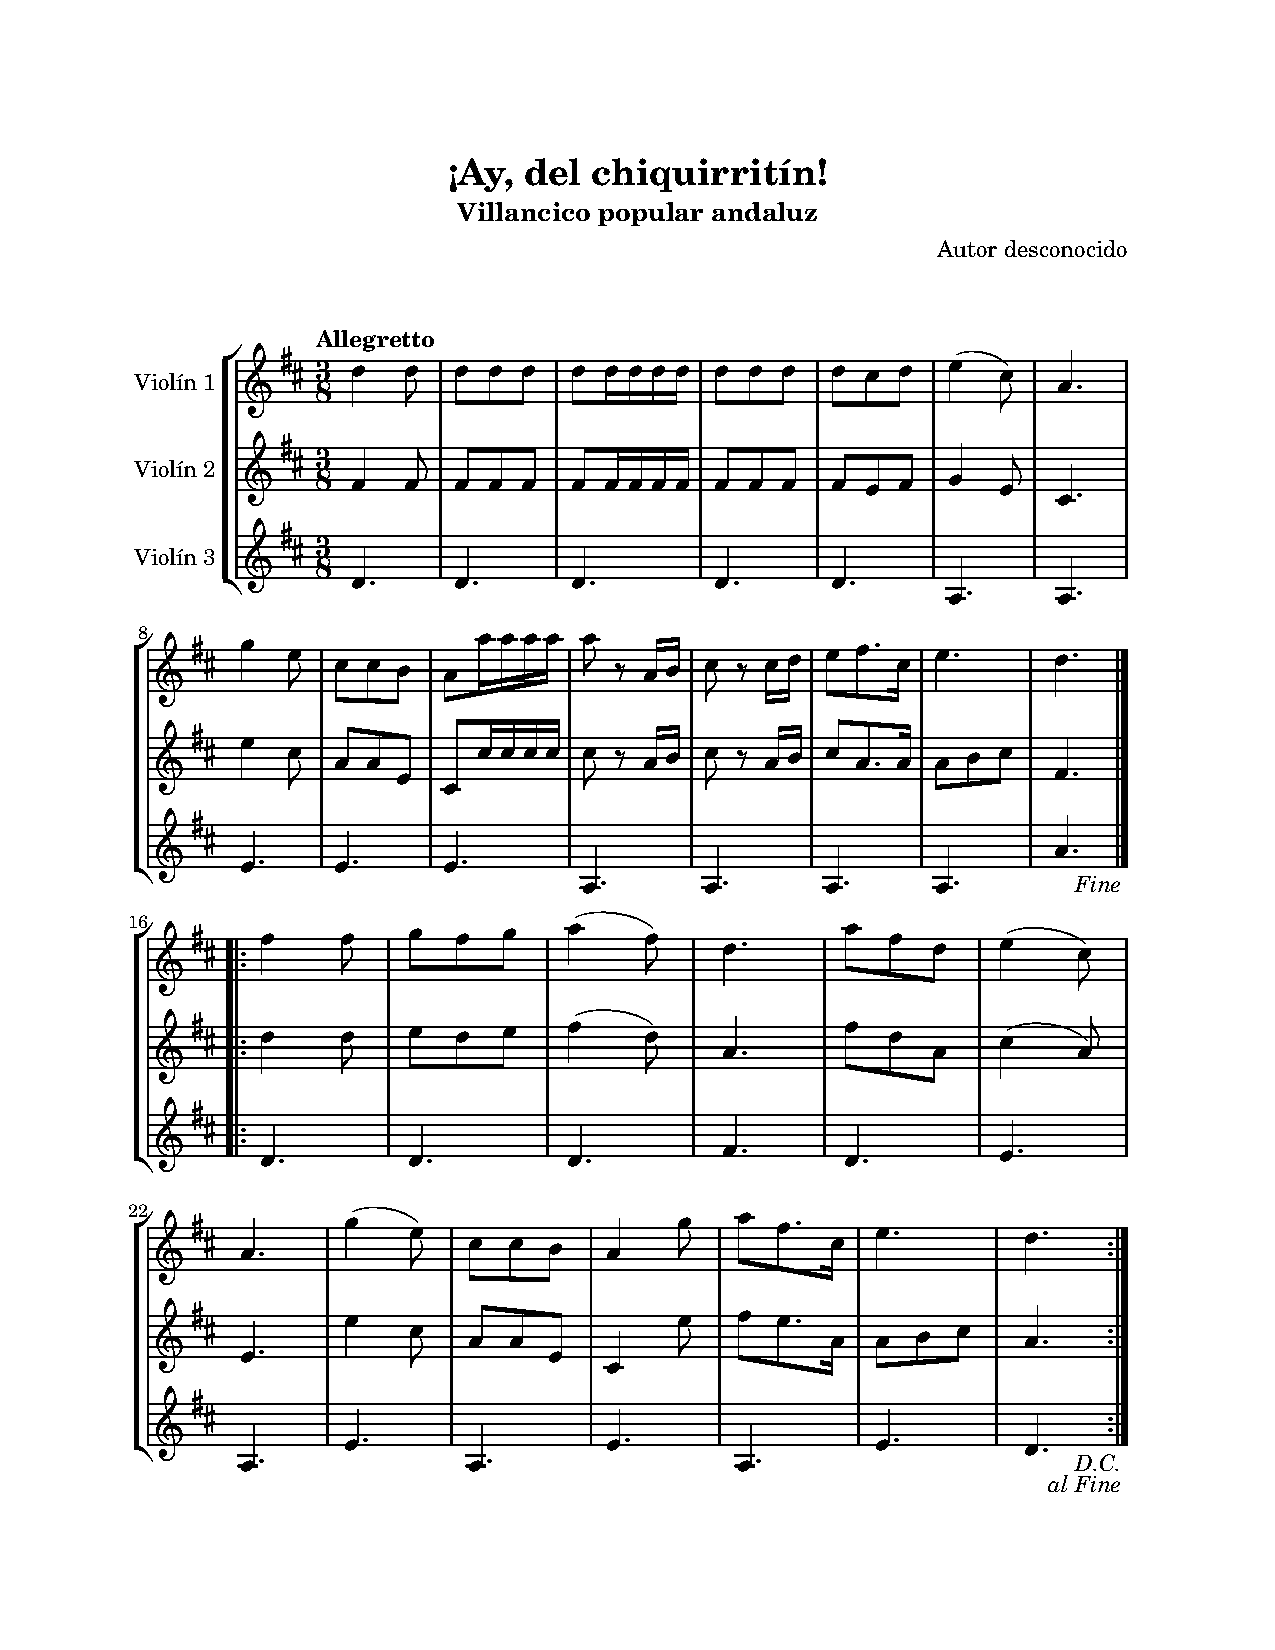
\includepdf[pages=-, pagecommand={\thispagestyle{plain}}]{ay-del-chiquirritin.pdf}

\includepdf[pages=-, pagecommand={\thispagestyle{plain}}]{la-marimorena.pdf}

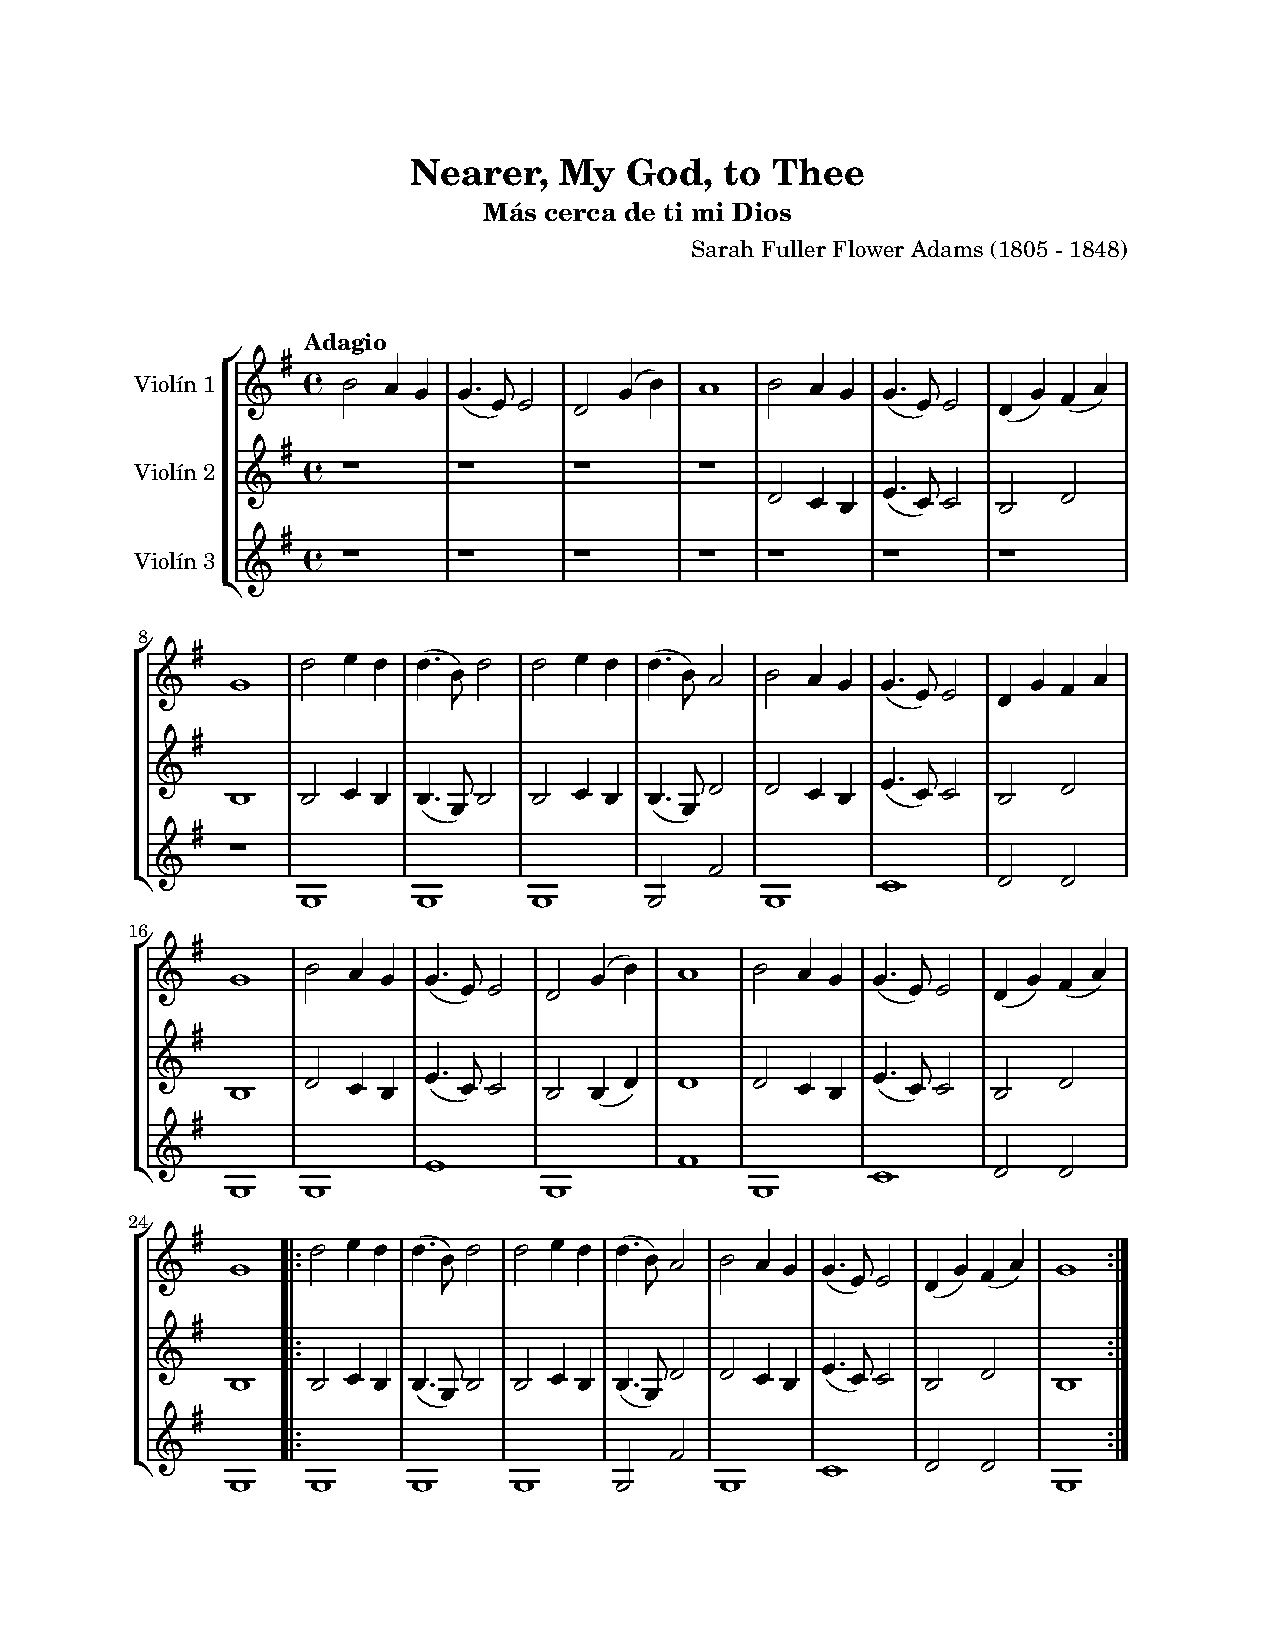
\includepdf[pages=-, pagecommand={\thispagestyle{plain}}]{nearer-my-god-to-thee.pdf}

\end{document}